\documentclass[a4paper,11pt] {ivoa}
\usepackage{geometry}                % See geometry.pdf to learn the layout
% options. There are lots.
\geometry{a4paper}                   % ... or a4paper or a5paper or ...
% \geometry{landscape}                % Activate for for rotated page geometry
% \usepackage[parfill]{parskip}    % Activate to begin paragraphs with an empty
% line rather than an indent
\usepackage{graphicx}
\usepackage{amssymb}
\usepackage{epstopdf}
\usepackage{amsmath}
\usepackage{hyperref}
\usepackage{color}
\usepackage{xcolor}
\usepackage{listings}

\DeclareGraphicsRule{.tif}{png}{.png}{`convert #1 `dirname #1`/`basename #1 .tif`.png}

\title{Implementing Note of the Framework built around PDL}
% Give author list: separate different authors with \\ 
% You can add email addresses with links \url{mailto:yourname@ivoa.net}
\author{Carlo Maria Zw\"olf}
\newcommand{\pdlversion}{0.1}
\newcommand{\pdldate}{\today}

%I have marked sections which I am unsure of with this
\newcommand{\tocheck}[1]{{\color{red} #1}}

% Give date and version number
\date{\pdldate}

% Choose one document type from below
%\ivoatype{IVOA Note}
\ivoatype{IVOA Working Draft}
%\ivoatype{IVOA Proposed Recommendation}
%\ivoatype{IVOA Recommendation}
\ivoagroup{GWS / Theory}
\version{\pdlversion}
\def\SVN$#1: #2 ${\expandafter\def\csname SVN#1\endcsname{#2}}
\SVN$Rev: 123 $

\urlthisversion{\pdlversion:  \pdldate\ (SVN Revision \SVNRev)}
\urllastversion{N/A}
\previousversion{
}

\begin{document}
\maketitle

\newpage

\tableofcontents

\newpage

\section{Introduction}\label{intro}
This document is a detailed and structured description (by this I means it is more user friendly than a JavaDoc) of the framework around PDL. In particular I explain how, starting from a PDL description, are implemented the automatic generation of validator algorithms and the dynamic Graphic User Interface (GUI). 

\section{The package structure}
I'm looking for a tool for generating a nice package dependency graph starting from the Eclipse project. If you have the solution, it is welcome...

\section{Java Objects corresponding to the PDL data Model}\label{Java_Objects}
These object 


are all generated using JAX-B on the PDL XML schema. The generated classes corresponds to the PDL 


\section{The CommonsObject package}\label{commons}
This package contains the classes 
\begin{itemize}
\item GeneralParameter.java
\item GeneralPatameterAlgebra.java
\end{itemize}

\subsection{The  GeneralParameter.java class }\label{generalParameter}
This class is the core PDL and is used for handling all the parameters. It is a way for encapsulating the usual basic types (integer, double, boolean, string) into an object. Moreover the modular design of this class allow users to easily define new types.\\

This attributes of this class are
\begin{itemize}
\item a field {\it value} of String type,\\
\item a field {\it type} of String type,\\
\item a field {\it description} of String type,\\
\item a field {\it visitor} of Ivisitor type (cf. paragraph \ref{visitor} for the definition of this interface).\\ 
\end{itemize}

The constructor of this class takes as arguments the quadruplet  {\it  value, type, description, visitor} and invoke the method {\it visit(GeneralParameter)} on the object we are creating. If all the test contained in the visitor (typically this methods verify if the value provided could be cast to the type contained into the {\it type} field) pass with no problem, then the object is created. If a problem is encountered, the constructor throws an {\it InvalidParameterException } exception explaining the reasons of the problem.\\

With this mechanisms, the validation of a GeneralParameter is automatically performed at its own construction. All the existing instances of GeneralParameter are natively validated. Moreover, just by modifying the content of the visitor class passed as arguments, developers could easily add support for new types. 

\subsection{The GeneralParameterAlgebra.java class}\label{gpalgebra}
This class is implemented using the singleton pattern. In the following, let $g_i$ be a family of GeneralParameter instances.
This class  contains the methods for computing:
\begin{itemize}
\item  the sum $g_r = g_i + g_j$;\\
\item the multiplication $g_r = g_i \cdot g_j$;\\
\item the difference of $g_r = g_i - g_j$. ;\\
For these last three items, if the both $g_i$ and $g_j$ are integer, the resulting GeneralParameter will be of integer type too. If one of the two is a real, then the result will be a real (this is internally hold using double types).\\
\item the power $g_r = g_i^{g_j}$. Since the native Java Math.pow method provide a double, the result will always 
be a GeneralParameter of real type;\\
\item the absolute value $|g_r|$. Since the native Math.abs method provide a double, the result will always be a GeneralParameter of real type;\\
\item the function $f(g_i)$, $\displaystyle f() \in \left\{ \sin() , \cos(), \tan(), \sin^{-1}(), \cos^{-1}(), \tan^{-1}(),  \exp(), \log() \right\}$. The result wil be a GeneralParamter of real type;
\item the sum of all the components $g_{i,j}$ of a vector of general parameters $\vec g_i$ : $g_r = \sum_j g_{i,j}$. By the choice of our implementation, the result is a GeneralParameter of real type;
\item the product of all the components $g_{i,j}$ of a vector of general parameters $\vec g_i$ : $g_r = \prod_j g_{i,j}$. By the choice of our implementation, the result is a GeneralParameter of real type;
\item the size of a vector $\vec g_i$. In this case the result is a generalParameter of type Intger and the incapsulated value will be the size of the vector.\\ 
\end{itemize} 
All  these operations (excepted the last one) are performed only if  $g_i$ (and $g_j$ too when it appears) is (are) numerical. In the other cases, this method will throw an InvalidExpression exception explaining the reasons of the problem;\\

\noindent Moreover this class contains methods for characterizing  instances of GeneralParameter:
\begin{itemize}
\item {\it areGeneralParameterEqual} takes $g_i$ and $g_j$ and return a boolean. This last is true if 
\begin{itemize}
\item both $g_i$, $g_j$ are numerical and the difference of the values $v(g_i)$ and $v(g_j)$ encapsulated in these objects is smaller than $\epsilon = 0.0000001$ ($v(g_i)-v(g_j)<\epsilon$), or 
\item the type of $g_i$  is equal (in the Java equalsIgnoreCase String sense) to the type of $g_j$ and the value if $g_i$ is equal (again, in the Java equalsIgnoreCase String sense) to the value of $g_j$.
\end{itemize} 
\item {\it isFirstGreaterThanSecond} takes $g_i$, $g_j$ and a boolean $r$. The result is true if 
\begin{itemize}
\item $r$ is true and $v(g_i) \geq v(g_j)$, or
\item $r$ is false and $v(g_i) > v(g_j)$.
\end{itemize}
\item {\it isFirstSmallerThanSecond} takes $g_i$, $g_j$ and a boolean $r$. The result is true if 
\begin{itemize}
\item $r$ is true and $v(g_i) \leq v(g_j)$, or
\item $r$ is false and $v(g_i) < v(g_j)$.
\end{itemize}
\item {\it isGeneralParameterInteger} takes $g_i$ and returns a boolean. This last is true if $v(g_i) \in \mathbb N$.
\item {\it isGeneralParameterReal} takes $g_i$ and returns a boolean. This last is true if $v(g_i) \in \mathbb R$.
\end{itemize}
 
 \section{The visitors package}\label{visitor}
This package contains the visitors classes used by the {\it GeneralParameter} class constructor (cf. paragraph \ref{generalParameter}).\\

\subsection{The visitors objects}
The interface {\it Ivisitor} describe the method {\it visit} which takes as argument the {\it GeneralParameter} instance to inspect.\\
The abstract {\it AbstractVisitor} class implements the {\it Ivisitor} interface. It defines 
\begin{itemize}
\item the abstract method {\it buildCriteriaList} which return a list of {\it Icriteria} (cf. par. \ref{criteria}). Developer has to implement this function in order to define his own list of criteria. By default, we provide the {\it GeneralParameterVisitor} class (cf. the end of this paragraph).
\item the {\it visit} function: the previous method is invoked and, for every {Icriteria} object returned, we verify if the couple (type, value) of the {\it GeneralParameter} instance passed as argument verify the criterion. If at least one criterion is satisfied, than the visit methods end positevely. If no criterion is satisfied, the methods throws an {\it InvalidParameterException} explaining the reasons of the problem.
\end{itemize}
The {\it GeneralParameterVisitor} class is the concrete implementation of {\it AbstractVisitor}. It defines the method {\it buildCriteriaList}. The list returned contains a {\it RealCriteria}, an {\it IntegerCriteria}, a {\it BooleanCriteria} and a {\it StringCriteria} (cf. par. \ref{criteria}).  

\subsection{The criteria objects}\label{criteria}
All the criteria we are going to define implements the {\it Icriteria} interface. This last describe the methods:
\begin{itemize}
\item {\it getAuthorizedCriteriaType}, which returns the String containing the type authorized by the concrete criterion implementing the interface.
\item {\it verifyCriteria}, which takes as argument a couple (type,value) characterizing a {\it GeneralParameter}. It returns the boolean true if the criterion is satisfied and false in the other case.
\end{itemize}
This interface is implemented by {\it RealCriteria}, an {\it IntegerCriteria}, a {\it BooleanCriteria} and a {\it StringCriteria}.

\subsubsection{The RealCriteria}
In this class, the method {\it getAuthorizedCriteriaType} returns the String ('real') {\bf used in the PDL grammar} for specifying that a parameter is of real type.\\
The {\it VerifyCriteria} method returns the boolean true if the type of the {\it GeneralParameter} is 'real' and if the value of the same  {\it GeneralParameter} could be cast to a double type with no errors. If the type of the  {\it GeneralParameter} is not 'real', this methods return false. Finally if the type of the {\it GeneralParameter} is 'real' and the value cannot be casted to a double, this method throws an {\it InvalidParameterException} explaining the reasons of the problem.

\subsubsection{The IntegerCriteria}
In this class, the method {\it getAuthorizedCriteriaType} returns the String ('Integer') {\bf used in the PDL grammar} for specifying that a parameter is of Integer type.\\
The {\it VerifyCriteria} method returns the boolean true if the type of the {\it GeneralParameter} is 'Integer' and if the value of the same  {\it GeneralParameter} could be cast to an Integer type with no errors. If the type of the  {\it GeneralParameter} is not 'Integer', this methods return false. Finally if the type of the {\it GeneralParameter} is 'Integer' and the value cannot be casted to an Integer, this method throws an {\it InvalidParameterException} explaining the reasons of the problem.

\subsubsection{The BooleanCriteria}
In this class, the method {\it getAuthorizedCriteriaType} returns the String ('Boolean') {\bf used in the PDL grammar} for specifying that a parameter is of Boolean type.\\
The {\it VerifyCriteria} method returns the boolean true if the type of the {\it GeneralParameter} is 'Boolean' and if the value of the same  {\it GeneralParameter} is equal to 'true' or 'false'. If the type of the  {\it GeneralParameter} is not 'Boolean', this methods return false. Finally if the type of the {\it GeneralParameter} is 'Boolean' and the value is not 'true' or 'false', this method throws an {\it InvalidParameterException} explaining the reasons of the problem.

\subsubsection{The StringCriteria}
In this class, the method {\it getAuthorizedCriteriaType} returns the String ('String') {\bf used in the PDL grammar} for specifying that a parameter is of String type.\\
The {\it VerifyCriteria} method returns the boolean true if the type of the {\it GeneralParameter} is 'String' and the boolean false in the other cases.

\section{The pdl.interpreter.expression package}\label{pdl.interpreter.expression}
In this package are contained all the classes for interpreting and parsing PDL expressions.\\
The entry point for understanding the expression interpreting mechanism is the abstract class {\it ExpressionParser}. 
It describes the abstract method {\it parse}, which interprets the expression invoking the method. The result of this method is a list of {\it GeneralParameter} instances. Since in PDL expressions are vectorial, the $i$-th element of that list corresponds to the result of the interpretation of $i$-th component of the vector expression.
The abstract class {\it ExpressionParser} is used, jointly with the polymorphism mechanism for building the {\it ExpressionParserFactory}

\subsection{The ExpressionParserFactory class}
This class is built by implementing the {\it singleton} pattern and is, as its name indicates, an implementation of the {\it factory} pattern.\\
The method {\it buildParser} takes as argument an instance of the PDL {\it Expression} object and returns an {\it ExpressionParser}.
More precisely, using introspection, this function analyze the instance of the PDL Expression:
\begin{itemize}
\item if the {\it Expression} is an instance of {\it AtomicConstantExpression} then the methods returns a {\it AtomicConstantExpressionParser};
\item if the {\it Expression} is an instance of {\it AtomicParameterExpression} then the methods returns a {\it AtomicParameterExpressionParser};
\item if the {\it Expression} is an instance of {\it FunctionExpression} then the methods returns a {\it FunctionExpressionParser};
\item if the {\it Expression} is an instance of {\it Function} then the methods returns a {\it FunctionParser};
\item if the {\it Expression} is an instance of {\it ParenthesisContent} then the methods returns a {\it ParenthesisContentParser};
\item if the {\it Expression} is not an instance of what seen in the previous items, the function throws an {\it InvalidExpression} exception.
\end{itemize} 
It is important to note that, since in PDL expressions are recursive, this factory will be invoked inside every concrete class implementing {\it ExpressionParser}.\\
In what follows, we are going to describe all these concrete classes returned by the  {\it buildParser} method (and implementing the {\it ExpressionParser}).


\subsection{The ExpressionWithPowerParser class}
This abstract class inherits from {\it ExpressionParser} and is used for factoring the code of all the classes interpreting PDL expressions involving powers. 
It specifies the method {\it evaluatePower} which takes as arguments two lists of {\it GeneralParameter}, one list for the base (let us note $g_i^{base}$ its elements) 
and the other for the exponent (let us note $g_i^{exp}$ its elements). This method returns:
\begin{itemize}
\item the base list of $g_i^{base}$, if the expos ant list is null;\\
\item the list whose elements are $\displaystyle \left(g_i^{base}\right)^{g_i^{exp}}$, if both lists have the same size. The power operation is performed in the {\it GeneralParameter} sense, using the methods described in paragraph \ref{gpalgebra}.
\item the list whose elements are  $\displaystyle \left(g_i^{base}\right)^{g_0^{exp}}$, if the exponent list contains only one element $g_0^{exp}$.
\end{itemize}
In the other cases, the  {\it evaluatePower} method throws and {\it InvalidExpression} exception, specifying the reasons of the problem.

\subsection{The AtomicParameterExpressionParser class}
This class extends the {\it ExpressionWithPowerParser} and is used for interpreting the PDL {AtomicParameterExpression} instances. Indeed this class has an attribute of type {\it AtomicParameterExpression} whose value is initialized by the class constructor.\\
In the overridden method {\it parse}, the following actions are performed:
\begin{itemize}
\item the instance of the SingleParameter referenced by the expression, is retrieved using the {\it Utilities} class methods.
\item if the power of the expression is not null, then we convert the power expression into a List of {\it GeneralParameter} by building (using the {\it ExpressionParserFactory}) the had hoc parser and invoking its {\it parse} method.
\item The expression (without the operation part) is evaluated: Using the {\it Utilities} class we get the list of {\it GeneralParameter} corresponding to the user provided input vector for the SingleParameter contained into the AtomicConstantExpression. We verify that the dimension of that list corresponds to the value put in the dimension field of the SingleParameter. If this test is negative we throws an {\it InvalidExpression} exception. If the test is positive, we invoke the method {\it evaluatePower} inherited from the {\it ExpressionWithPowerParser} superclass. 
\item If the {\it Operation} contained into the {\it AtomicParameterExpression} is not null, we evaluate the results of this operation (cf \ref{operationParser}, the result of the expression without the operation is in this case our first operand).
\item Finally, the methods returns the list of {\it GeneralParameter} resulting from the previous stages.  
\end{itemize}

\subsection{The AtomicConstantExpressionParser class}
This class extends the {\it ExpressionWithPowerParser} and is used for interpreting the PDL {AtomicConstantExpression} instances. Indeed this class has an attribute of type {\it AtomicConstantExpression} whose value is initialized by the class constructor.\\
In the overridden method {\it parse}, the following actions are performed:
\begin{itemize}
\item If the power of the expression is not null, then we convert the power expression into a List of {\it GeneralParameter} by building (using the {\it ExpressionParserFactory}) the had hoc parser and invoking its {\it parse} method.
\item The expression (without the operation part) is evaluated: first we recover the set of constant values provided in the description of  the AtomicConstantExpression. Then we try to instantiate a list of {\it GeneralParameter} whose values are the previously retrieved and the type is the one contained into the ConstantType attribute (of type ParameterType) contained into the AtomicConstantExpression. If no exception is thrown during this process, the method {\it evaluatePower} (inherited from the {\it ExpressionWithPowerParser} superclass) is invoked.
\item If the {\it Operation} contained into the {\it AtomicConstantExpression} is not null, we evaluate the results of this operation (cf \ref{operationParser}, the result of the expression without the operation is in this case the first operand).
\item Finally, the methods returns the list of {\it GeneralParameter} resulting from the previous stages.
\end{itemize}

\subsection{The ParenthesisContentParser class}
This class extends the {\it ExpressionWithPowerParser} and is used for interpreting the PDL {\it  ParenthesisContent} expression instances. This class has an attribute of type {\it ParenthesisContent} whose value is initialized by the class constructor.\\
In the overridden method {\it parse}, the following actions are performed:
\begin{itemize}
\item The expression 'contained into the parenthesis', i.e. with the highest priority, is first evaluated by calling the {\it ExpressionParserFactory} and invoking on its returned object the method {\it parse}.
\item  If the power of the expression is not null, then we convert the power expression into a List of {\it GeneralParameter} by building (using the {\it ExpressionParserFactory}) the had hoc parser and invoking its {\it parse} method.
\item The expression (without the operation part) is evaluated:  the method {\it evaluatePower} (inherited from the {\it ExpressionWithPowerParser} superclass) is invoked using as base the list of {\it GeneralParameter} corresponding to the expression contained into the parenthesis and as exponent the list of {\it GeneralParameter} corresponding to the power.
\item  If the {\it Operation} contained into the {\it ParenthesisContent}  is not null, we evaluate the results of this operation (cf \ref{operationParser}, the result of the expression without the operation is in this case the first operand).
\item Finally, the methods returns the list of {\it GeneralParameter} resulting from the previous stages.
\end{itemize}

\subsection{The FunctionParser class}
This class extends the {\it ExpressionParser} and is used for interpreting PDL {\it Function} expressions.\\
This class has an attribute of type {\it Function} whose value is initialized by the class constructor.\\
In the overridden method {\it parse}, the following actions are performed:
\begin{itemize}
\item The argument of the function is interpreted by invoking by calling the {\it ExpressionParserFactory} and invoking on its returned object the method {\it parse};
\item According to the function type contained in the attribute {\it functionName} of the {\it Function} object, we invoke the good correspondent method contained into the {GeneralParameterAlgebra} class (cf. \ref{gpalgebra})  passing the list of {\it GeneralParameter} (built during the previous step) as argument. The result of this invocation is returned by the function.
\end{itemize}

\subsection{The FunctionExpressionParser class}
This class extends the {\it ExpressionWithPowerParser} and is used for interpreting the PDL {\it  FunctionExpression} expression instances. This class has indeed an attribute of type {\it FunctionExpression} whose value is initialized by the class constructor.\\
In the overridden method {\it parse}, the following actions are performed:
\begin{itemize}
\item The {\it Function} contained into the FunctionExpression is interpreted by calling the {\it ExpressionParserFactory} and invoking on its returned object the method {\it parse};
\item  If the power of the expression is not null, then we convert the power expression into a List of {\it GeneralParameter} by building (using the {\it ExpressionParserFactory}) the had hoc parser and invoking its {\it parse} method.
\item The expression (without the operation part) is evaluated:  the method {\it evaluatePower} (inherited from the {\it ExpressionWithPowerParser} superclass) is invoked using as base the list of {\it GeneralParameter} corresponding to the {\it Function} expression contained into the {\it FunctionExpression} expression  and as exponent the list of {\it GeneralParameter} corresponding to the power.
\item  If the {\it Operation} contained into the {\it ParenthesisContent}  is not null, we evaluate the results of this operation (cf \ref{operationParser}, the result of the expression without the operation is in this case the first operand).
\item Finally, the methods returns the list of {\it GeneralParameter} resulting from the previous stages.
\end{itemize}

\subsection{The OperationParser class}\label{operationParser}
This class is used for interpreting the results of operations expressed in PDL syntax. 
This class has indeed an attribute of {\it Operation} type, whose value is initialized by the class constructor. The only method of this class is {\it processOperation}, which takes as argument a list of {\it GeneralParameter} representing the first operand of the operation. In this last method, the following operations are performed:
\begin{itemize}
\item The second operand of the operation (i.e. the {\it Expression} instance contained into the {\it Operation} object) is interpreted by calling the {\it ExpressionParserFactory} and invoking on its returned object the method {\it parse};
\item We get the {\it OperationType} from the  {\it Operation} object and invoke the good corresponding method contained into the {GeneralParameterAlgebra} class (cf. \ref{gpalgebra})  passing the {\it GeneralParameter} list corresponding to the first and second operands as arguments. The function returns the result of this last invokation.
\end{itemize}

\section{The pdl.interpreter.condition package}\label{conditionInterpreters}
In this package we put all the classes used for interpreting the instances of all the PDL objects implementing {\it AbstractCondition}.\\
The entry point for understanding the mechanisms of this package is the abstract class {\it ConditionInterpreter}. This last describe the abstract method
{\it isConditionVerified}  which a boolean value. True id the condition is verified, false in the opposite case. This method could throws three kind of exceptions: {\it InvalidExpression,  InvalidParameterException, InvalidCondition}.\\
The abstract class {\it ConditionInterpreter} is used, jointly with the polymorphism mechanism for building the {\it ConditionInterpreterFactory}

\subsection{The ConditionInterpreterFactory class}\label{conditionInterpreterFactory}
This class is built by implementing the {\it singleton} pattern and is, as its name indicates, an implementation of the {\it factory} pattern.\\
The method {\it buildConditionInterpreter} takes as argument an instance of the PDL {\it AbstractCondition} object and returns a {\it ConditionInterpreter}.
More precisely, using introspection, this function analyze the instance of the PDL Expression:
\begin{itemize}
\item if the {\it AbstractCondition} is an instance of {\it ValueLargerThan} then the methods returns a {\it ValueLargerThanInterpreter};
\item if the {\it AbstractCondition} is an instance of {\it ValueSmallerThan} then the methods returns a {\it ValueSmallerThanInterpreter};
\item if the {\it AbstractCondition} is an instance of {\it ValueInRange} then the methods returns a {\it ValueInRangeInterpreter};
\item if the {\it AbstractCondition} is an instance of {\it ValueDifferentFrom} then the methods returns a {\it ValueDifferentFromInterpreter};
\item if the {\it AbstractCondition} is an instance of {\it BelongToSet} then the methods returns a {\it BelongToSetInterpreter};
\item if the {\it AbstractCondition} is an instance of {\it DefaultValue} then the methods returns a {\it DefaultValueInterpreter};
\item if the {\it AbstractCondition} is an instance of {\it IsInteger} then the methods returns a {\it IsIntegerInterpreter};
\item if the {\it AbstractCondition} is an instance of {\it IsReal} then the methods returns a {\it IsRealInterpreter};
\item if the {\it AbstractCondition} is an instance of {\it IsNull} then the methods returns a {\it IsNullInterpreter};
\item if the {\it AbstractCondition} is not an instance of what seen in the previous items, the function throws an {\it InvalidCondition} exception, explaining the origin of the problem.
\end{itemize} 
In what follows, we are going to describe all these concrete classes returned by the  {\it buildConditionInterpreter} method (and implementing the {\it ConditionInterpreter}).

\subsection{The ValueLargerThanInterpreter class}\label{VLT}
This class extends the  {\it ConditionInterpreter} and is used for interpreting the {\it ValueLargerThan} PDL condition. Indeed this class has an attribute of type {\it ValueLargerThan} whose value is initialized by the class constructor. \\
In the overridden {\it isConditionVerified} method, the following actions are performed:
\begin{itemize}
\item We build $\vec g^{exp}$, the list of {\it GeneralParameter} resulting from the interpretation of the {\it Expression} passed as argument to the function (by calling the {\it ExpressionParserFactory} and invoking on its returned object the method {\it parse}).
\item We build $\vec g^{cond}$, the list of {\it GeneralParameter} resulting from the interpretation of the {\it Expression} contained into the field {\it Value} of the {\it ValueLargerThan} condition.
\item If the lists built during the two previous steps has different sizes, we throw a {\it InvalidCondition} expression expelling the problem origin. 
\item For every couple $(g_i^{exp}, g_i^{cond})$ we call the method  {\it isFirstGreaterThanSecond} of {\it GeneralParameterAlgebra} (by setting the boolean field reached according to the value contained in the attribute {\it reached} in the  {\it ValueLargerThan} condition, cf. paragraph \ref{gpalgebra}). The method returns the true boolean value if and only if all the results of this calls are true for all the couples. It returns false otherwise. 
\end{itemize}

\subsection{The ValueSmallerThanInterpreter class}\label{VST}
This class extends the  {\it ConditionInterpreter} and is used for interpreting the {\it ValueSmallerThan} PDL condition. Indeed this class has an attribute of type {\it ValueSmallerThan} whose value is initialized by the class constructor. \\
In the overridden {\it isConditionVerified} method, the following actions are performed:
\begin{itemize}
\item We build $\vec g^{exp}$, the list of {\it GeneralParameter} resulting from the interpretation of the {\it Expression} passed as argument to the function (by calling the {\it ExpressionParserFactory} and invoking on its returned object the method {\it parse}).
\item We build $\vec g^{cond}$, the list of {\it GeneralParameter} resulting from the interpretation of the {\it Expression} contained into the field {\it Value} of the {\it ValueLargerThan} condition.
\item If the lists built during the two previous steps has different sizes, we throw a {\it InvalidCondition} expression expelling the problem origin. 
\item For every couple $(g_i^{exp}, g_i^{cond})$ we call the method  {\it isFirstSmallerThanSecond} of {\it GeneralParameterAlgebra} (by setting the boolean field reached according to the value contained in the attribute {\it reached} in the  {\it ValueSmallerThan} condition, cf. paragraph \ref{gpalgebra}). The method returns the true boolean value if and only if all the results of this calls are true for all the couples. It returns false otherwise. 
\end{itemize}

\subsection{The ValueInRangeInterpreter class}
This class extends the  {\it ConditionInterpreter} and is used for interpreting the {\it ValueInRange} PDL condition. Indeed this class has an attribute of type {\it ValueSmallerThan} whose value is initialized by the class constructor. \\
In the overridden {\it isConditionVerified} method, the following actions are performed:
\begin{itemize}
\item We interpret the {\it Sup} field of the  {\it ValueInRange}, which is of type {\it ValueSmallerThan} (cf. par. \ref{VST})
\item We interpret the {\it Inf} field of the  {\it ValueInRange}, which is of type {\it ValueLargerThan} (cf. par. \ref{VLT})
\item We returns true if both the previous interpretations returned true, false otherwise.
\end{itemize}

\subsection{The BelongToSetInterpreter class}
This class extends the  {\it ConditionInterpreter} and is used for interpreting the {\it BelongToSet} PDL condition. Indeed this class has an attribute of type {\it BelongToSet} whose value is initialized by the class constructor. \\
In the overridden {\it isConditionVerified} method, the following actions are performed:
\begin{itemize}
\item We build $\vec g^{exp}$, the list of {\it GeneralParameter} resulting from the interpretation of the {\it Expression} passed as argument to the function (by calling the {\it ExpressionParserFactory} and invoking on its returned object the method {\it parse}).
\item For every expression $value_j$ appearing in the field {\it Value} of the {\it BelongToSet} object
\begin{itemize}
\item  We interpret $value_j$, by calling the {\it ExpressionParserFactory} and invoking on its returned object the method {\it parse}. Let $\vec g^{value_j}$ be this result.
\item If the list $\vec g^{value_j}$ resulting from this interpretation is equal to $\vec g^{exp}$ (i.e. $\forall i$, $g_i^{exp}=g_i^{value_j}$ in the sense defined by the method {\it areGeneralParameterEqual} of {\it GeneralParameterAlgebra}, cf. par. \ref{gpalgebra} ), then the function returns true. False otherwise. 
\end{itemize}
\end{itemize}

\subsection{The ValueDifferentFromInterpreter class}
This class  extends the  {\it ConditionInterpreter} and is used for interpreting the {\it ValueDifferentFrom} PDL condition. Indeed this class has an attribute of type {\it ValueDifferentFrom} whose value is initialized by the class constructor. \\
In the overridden {\it isConditionVerified} method, the following actions are performed:
\begin{itemize}
\item We build $\vec g^{exp}$, the list of {\it GeneralParameter} resulting from the interpretation of the {\it Expression} passed as argument to the function (by calling the {\it ExpressionParserFactory} and invoking on its returned object the method {\it parse}). 
\item We build $\vec g^{value}$, the list of  {\it GeneralParameter} resulting from the interpretation of the {\it Expression} contained into the field {\it Value} of the  {\it ValueDifferentFrom} object.
\item The methods return the boolean true if, at least for a given of $i$, we have $g_i^{exp} \neq g_i^{value}$.
\end{itemize}

\subsection{The IsRealInterpreter class}
This class  extends the  {\it ConditionInterpreter} and is used for interpreting the {\it IsReal} PDL condition. In the overridden {\it isConditionVerified} method, the following actions are performed:
\begin{itemize}
\item We build $\vec g^{exp}$, the list of {\it GeneralParameter} resulting from the interpretation of the {\it Expression} passed as argument to the function (by calling the {\it ExpressionParserFactory} and invoking on its returned object the method {\it parse}). 
\item The method returns the boolean true if for all $i$, $g_i^{exp}$ is real (the test is performed by calling the method {\it isGeneralParameterReal} of the {\it GeneralParameterAlgebra} class, cf. par. \ref{gpalgebra}).
\end{itemize}

\subsection{The IsIntegerInterpreter class}
This class  extends the  {\it ConditionInterpreter} and is used for interpreting the {\it IsInteger} PDL condition. In the overridden {\it isConditionVerified} method, the following actions are performed:
\begin{itemize}
\item We build $\vec g^{exp}$, the list of {\it GeneralParameter} resulting from the interpretation of the {\it Expression} passed as argument to the function (by calling the {\it ExpressionParserFactory} and invoking on its returned object the method {\it parse}). 
\item The method returns the boolean true if for all $i$, $g_i^{exp}$ is integer (the test is performed by calling the method {\it isGeneralParameterInteger} of the {\it GeneralParameterAlgebra} class, cf. par. \ref{gpalgebra}).
\end{itemize}

\subsection{The IsNullInterpreter class}
This class  extends the  {\it ConditionInterpreter} and is used for interpreting the {\it IsNull} PDL condition. \\
It is important to remark that, due to the signification of the {\it IsNull} condition, this last could be applied only on {\it AtomicParameterExpression} (because it has sense to say parameter $p_1$ is null, but has no sense to say $(p_1 \cdot p_2 / p_3)$ is null.\\
In the overridden {\it isConditionVerified} method, the following actions are performed:
\begin{itemize}
\item If the {\it Expression} passed as parameter is not an {\it AtomicParameterExpression} we throw an {\it InvalidCondition} exception, explaining the problem source.
\item We get the {\it SingleParameter} instance from the {\it ParameterReference} contained into the {\it Expression}.
\item We look\footnote{by calling the {\it getuserProvidedValuesForParameter} of the {\it Utilities} class} for the value (or values for vector Parameter cases) provided by user for the {\it SingleParameter}. If no value is provided, the method return true. Otherwise, it returns false.
\end{itemize}

\subsection{The DefaultValueInterpreter class}
This class extends the {\it ConditionInterpreter} and is used in association {\it DefaultValue} PDL condition. \\
Since this particular condition don't need to be interpreted as the previous ones (it is used only for saying that the default value of a parameter is a given value) the overridden method  {\it isConditionVerified}  always returns true.

\section{The pdl.interpreter.criterion package}
In this package we put all the classes used for interpreting instances of all the PDL objects implementing {\it AbstractCriterion}.
The entry point for understanding the mechanism of this package is the abstract class {\it AbstractCriterionInterpreter}.
This last describe the abstract method {\it isCriterionSatisfied} which returns a boolean value: true if the criterion is satisfied, false in the opposite case. This method could throw four kind of exceptions: {\it InvalidExpression, InvalidParameterException, InvalidCondition, InvalidCriterion}.\\
The class  {\it AbstractCriterionInterpreter} is used, jointly with the polymorphism mechanism for building the {\it CriterionInterpreterFactory}.

\subsection{The CriterionInterpreterFactory class}\label{criterionFactory}
This class is built by implementing the {\it singleton} pattern and is, as its name indicates, an implementation of the {\it factory} pattern.\\
The method {\it buildCriterrionInterpreter} takes as argument an instance of the PDL {\it AbstractCriterion} object and returns a {\it AbstractCriterionInterpreter}.
More precisely, using introspection, this function analyze the instance of the PDL Expression:
\begin{itemize}
\item if the {\it AbstractCriterion} is an instance of {\it Criterion} then the methods returns a {\it CriterionInterpreter};
\item if the {\it AbstractCriterion} is an instance of {\it ParenthesisCriterion} then the methods returns a {\it ParenthesisCriterion};
\item if the {\it AbstractCriterion} is not an instance of what seen in the previous items, the function throws an {\it InvalidCriterion} exception, explaining the origin of the problem.
\end{itemize} 
In what follows, we are going to describe these two concrete classes returned by the  {\it buildCriterrionInterpreter} method (and implementing the {\it AbstractCriterionInterpreter}).

\subsection{The CriterionInterpreter class}
This class  extends the  {\it AbstractCriterionInterpreter} and is used for interpreting the {\it Criterion} PDL criterion. \\
Indeed this class has an attribute of type {\it Criterion} whose value is initialized by the class constructor. \\
In the overridden {\it isCriterionSatisfied} method, the following actions are performed:
\begin{itemize}
\item We interpret the condition {\it ConditionType} contained into the {\it Criterion} object.
For this we call the method {\it buildConditionInterpreter} of  {\it ConditionInterpreterFactory} (cf. par \ref{conditionInterpreterFactory}). We call the method {\it isConditionVerified} (cf. par. \ref{conditionInterpreters}) contained in the object returned by {\it buildConditionInterpreter} by passing as argument the {\it Expression} contained into the {\it Criterion} object. This returns the boolean value $b_1$.
\item If the {\it Criterion} object has no {\it LogicalConnector}, we return the boolean obtained at the previous item. 
\item If the {\it Criterion} object has a {\it LogicalConnector}, we interpret it (as explained in paragraph \ref{logicalConnectorInt}), by passing to the method {\it interpret} of {\it LogicalConnectorInterpreter}  $b_1$ as parameter. Then the method returns the result of this last interpretation.
\end{itemize}

\subsection{The ParenthesisCriterionInterpreter class}
This class extends the {\it AbstractCriterionInterpreter} and is used for interpreting the {\it ParenthesisCriterion} PDL object. Indeed it contains an attribute of type {\it ParenthesisCriterion} whose value is initialized by the class constructor. We recall that in PDL syntax, the {\it ParenthesisCriterion} are used for defining complex criteria, with arbitrary evaluation priority fixed by the user. \\
In the overridden method {\it isCriterionSatisfied} the following actions are performed:
\begin{itemize}
\item The {\it AbstractCriterion} contained into the {\it ParenthesisCriterion} is interpreted  by calling the method {\it isCriterionSatisfied} contained into the object returned by the method {\it buildCriterionInterpreter} (of the class {\it CriterionInterpreterFactory}, cf. par. \ref{criterionFactory}). Let $b_1$ be the boolean result of this interpretation.
\item If the {\it ParenthesisCriterion} has no {\it ExternalLogicalCriterion}, the method returns $b_1$.
\item If the {\it ParenthesisCriterion} has no {\it ExternalLogicalCriterion}, the methods return the boolean resulting from the call of the method 
\end{itemize}

\subsection{The LogicalConnectorInterpreter class}\label{logicalConnectorInt}
This class is used for interpreting the abstract {\it LogicalConnector} objects. Indeed, it contains an attribute of {\it LogicalConnector} type. We recall that the two concrete classes implementing {\it LogicalConnector} are {\it And} and {\it Or}.\\
The method {\it interpret} takes as argument a boolean value $b_1$ (which is  typically the result of the interpretation of a first Criterion, which contains the {\it LogicalConnector} we are trying to interpret) and returns a boolean value. The following actions are performed inside this method:
\begin{itemize}
\item The second criterion (i.e. the criterion contained into the {LogicalConnector} instance) is interpreted by calling the method {\it isCriterionSatisfied} contained into the object returned by the method {\it buildCriterionInterpreter} (of the class {\it CriterionInterpreterFactory}, cf. par. \ref{criterionFactory}). Let $b_2$ be the result of this interpretation.
\item If the instance of {\it LogicalConnector} is of type {\it And}, the boolean $(b_1 \mbox{ and } b_2)$ is returned.
\item If the instance of {\it LogicalConnector} is of type {\it Or}, the boolean $(b_1 \mbox{ or } b_2)$ is returned.
\end{itemize}

\section{The pdl.interpreter.conditionalStatement package}
In this package we put all the classes used for interpreting the instances of all the PDL objects implementing {\it ConditionalStatement}.\\
The entry point for understanding the mechanisms of this package is the abstract class {\it ConditionalStatementInterpreter}. This last describe two abstract methods
\begin{itemize}
\item {\it isStatementSwitched} which returns a boolean value: true if the statement is switched (i.e. if we are in a case where the statement has to be considered), false otherwise.
\item {\it isValidStatement} which returns a boolean value: true if the statement is valid, false otherwise.
\end{itemize}
The abstract class {\it ConditionalStatementInterpreter} is used, jointly with the polymorphism mechanism for building the {\it ConditionalStatementInterpreterFactory}.

\subsection{The ConditionalStatementInterpreterFactory class}\label{statementFactory}
This class is built by implementing the {\it singleton} pattern and is, as its name indicates, an implementation of the {\it factory} pattern.\\
The method {\it buildInterpreter} takes as argument an instance of the PDL {\it ConditionalStatement} object and returns a {\it ConditionalStatementInterpreter}.
More precisely, using introspection, this function analyze the instance of the PDL Expression:
\begin{itemize}
\item if the {\it ConditionalStatement} is an instance of {\it AlwaysConditionalStatement} then the methods returns a {\it AlwaysConditionalStatementInterpreter};
\item if the {\it ConditionalStatement} is an instance of {\it IfThenConditionalStatement} then the methods returns a {\it IfThenConditionalStatementInterpreter};
\item if the {\it ConditionalStatement} is not an instance of what seen in the previous items, the function throws an {\it InvalidConditionalStatement} exception, explaining the origin of the problem.
\end{itemize} 
In what follows, we are going to describe these two concrete classes returned by the  {\it buildInterpreter} method (and implementing the {\it ConditionalStatementInterpreter}).

\subsection{The AlwaysConditionalStatementInterpreter class}
This class extends the {\it ConditionalStatementInterpreter} and is used for interpreting the {\it AlwaysConditionalStatement} PDL objects. Indeed this class has an attribute of {\it AlwaysConditionalStatement} type, whose value is initialized by the class constructor. Moreover it contains a boolean attribute {\it isStatementSwitched} which is set to true by the class constructor, since as the name indicates an {\it AlwaysConditionalStatement} is always valid and has no conditions to be verified.\\
\begin{itemize}
\item The overridden method {\it isStatementSwitched} is a getter on the  {\it isStatementSwitched} and always returns true.
\item The overridden method {\it isValidStatement} calls the method {\it buildCriterionInterpreter} of the factory class {\it CriterionInterpreterFactory} (cf. par. \ref{criterionFactory}) by passing as argument the PDL {\it Criterion} object contained into the {\it Always} PDL object\footnote{implementing the PDL abstract class {\it ConditionalClause}}, which is in turn contained into the {\it AlwaysConditionalStatement} class attribute. The function returns the result of the method {\it isCriterionSatisfied} owned by the object returned by the {\it buildCriterionInterpreter} method.
\end{itemize}

\subsection{The IfThenConditionalStatementInterpreter class}
This class extends the {\it ConditionalStatementInterpreter} and is used for interpreting the {\it IfThenConditionalStatement} PDL objects. Indeed this class has an attribute of {\it IfThenConditionalStatement} type, whose value is initialized by the class constructor. Moreover it contains a boolean attribute {\it isStatementSwitched} whose value is computed by the method {\it isStatementSwitched}.\\
\begin{itemize}
\item In the overridden method {\it isStatementSwitched} the following actions are performed:
\begin{itemize}
\item We call the method {\it buildCriterionInterpreter} of the factory class {\it CriterionInterpreterFactory} (cf. par. \ref{criterionFactory}) by passing as argument the PDL {\it Criterion} object contained into the {\it If} PDL object (which is in turn contained into the {\it IfThenConditionalStatement} class attribute). If no exception is detected, the function returns the result of the method {\it isCriterionSatisfied} owned by the object returned by the {\it buildCriterionInterpreter} method.
\item In case of exception, we are not able to evaluate the condition, this means that the statement is not switched: the function return the boolean false.\\
\end{itemize}
\item In the overridden method the following actions are performed:
\begin{itemize}
\item The class attribute {\it isStatementSwitched} is set with the value returned by the  {\it isStatementSwitched} method.
\item If the statement is not switched, the function returns true: indeed if the statement is not switched it is always valid, since the contained condition has no matter.
\item If the the statement is switched, it is valid only if the criterion contained into the {\it Then} PDL condition (which is in turn contained into the class attribute of type {\it IfThenConditionalStatement}) is valid. Indeed the function calls the method {\it buildCriterionInterpreter} of the factory class {\it CriterionInterpreterFactory} (cf. par. \ref{criterionFactory}) by passing as argument the PDL {\it Criterion} object contained into the {\it Then} PDL object . The function returns the result of the method {\it isCriterionSatisfied} owned by the object returned by the {\it buildCriterionInterpreter} method.
\end{itemize}
\end{itemize}

\subsection{The StatementHelperContanier class}\label{StatementHelperContainer}
This class is a Java Bean used for easily handling the properties of the {\it ConditionalStatement} objects. It is used for facilitating communications between the logical layers we explained into the previous paragraphs and the IHM layer. It contains the 
\begin{itemize}
\item {\it StatementComment} String attribute. It is used for storing the comments contained into the attribute {\it comment} of all {\it ConditionalStatement} objects.
\item {\it statementSwitched} boolean attribute,
\item {\it statementValid} boolean attribute,
\item {\it statement} attribute of type {\it ConditionalStatement},
\end{itemize}
and their related getters and setters.

\section{The pdl.interpreter.groupInterpreter package}
In this package we put all the classes used for interpreting the {\it ParameterGroup} objects.\\
This package contains two classes
\begin{itemize}
\item {\it GroupHandlerHelper} which plays a role analogous to the {\it StatementHelperContainer} class (cf. par. \ref{StatementHelperContainer}).
\item {\it GroupProcessor} which implements the business logic for processing all the group of a given PDL service.
\end{itemize}

\subsection{The GroupHandlerHelper class}\label{GroupHandlerHelper}
This class is used for easily handling properties of {\it ParameterGroup} objects. It contains the following attributes
\begin{itemize}
\item the String {\it fatherName} which indicates the name of the direct ancestor of the current group,
\item the List of String {\it sonNames} which indicates the name of the direct offsprings of the current group,
\item the String {\it groupName} which indicates the name of the current group,
\item the {\it ParameterGroup} {\it group} which is the current group,
\item the List of {\it SingleParameter} objects {\it singleParamsIntoThisGroup} which indicates the {\it SingleParameter} instances contained into the current group, 
\item the boolean {\it groupValid} which indicates if all the {\it ConditionalStatement} contained into the {\it ConstraintOnGroup} object of the current group are valid,
\item the List of {\it StatementHelperContainer} objects {\it statementHelperList}, which associates to any {\it ConditionalStatement} contained into the {\it ConstraintOnGroup} object of the current group, the corresponding  {\it StatementHelperContainer}.
\end{itemize}
With the exception of {\it setGroup} method, all the getters and setters associated to these attributes are usual.\\ 
In {\it setGroup}, first we set the attribute {\it group} according to the value passed as argument. Then we set  the {\it groupName} and, by invoking the method {\it getParameterForTheGroup} of  the {\it Utilities} class, the attribute {\it singleParamsIntoThisGroup}.

\subsection{The GroupProcessor class}\label{groupProcessor}
As already mentioned, this class implements the logic for processing the groups of a given PDL service.\\
This class has two attributes 
\begin{itemize}
\item {\it service} of type the PDL {\it Service},
\item {\it groupsHandler} which is a List of {\it GroupHandlerHelper} objects  (cf. par. \ref{GroupHandlerHelper}), one for every {\it ParameterGroup} of the {\it service},
\end{itemize}
two public methods
\begin{itemize}
\item {\it getGroupsHandler}, an usual getter on the {\it groupsHandler} attribute,
\item  {\it process} which process the groups of parameters composing the service, 
\end{itemize}
and three private methods
\begin{itemize}
\item {\it buildGroupListFromService}, which builds the group structure from the PDL {\it Service},
\item {\it addGroups}, which adds a particular group to the  {\it groupsHandler} List,
\item {\it processStatementsOfGroups}, which process and interoperate all the {\it ConditionalStatment} contained into the {\it ConstraintOnGroup} object all the groups composing the service.
\end{itemize}
In the following we are going to explain in details the actions performed in these methods.

\subsubsection{The process method}\label{process}
This void method, which takes no argument, initializes the value of the attribute {\it groupsHandler} by calling the method 
{\it buildGroupListFromService} (cf. par. \ref{buildGroupListFromService}) then call the method {\it processStatementsOfGroups} (cf. par. \ref{processStatementsOfGroups}).
 
\subsubsection{The buildGroupListFromService method}\label{buildGroupListFromService}
This method, which takes no argument, returns a List of {\it GroupHandlerHelper} objects. After initializing the list to be returned, it calls the 
{\it addGroups} method\footnote{Pay attention: the method {\it addGroups} will modify the list it receives as argument} (cf. par. \ref{addGroups}), by passing as arguments 
\begin{itemize}
\item the list that will be returned, 
\item the {\it Input} object of type {\it ParameterGroup} contained into the PDL {\it Service},
\item the String 'root'.
\end{itemize}

\subsubsection{The addGroups method}\label{addGroups}
This void method has a recursive structure. It takes as arguments 
\begin{itemize}
\item a List of {\it GroupHandlerHelper} (this list will be modified by the function),
\item a {\it ParameterGroup} PDL object,
\item a String containing the name of the father of this {\it ParameterGroup}.
\end{itemize}
In this method, the following actions are performed:
\begin{itemize}
\item A temporary {\it GroupHandlerHelper} is created. Its attribute {\it group} is set to the value passed as second argument and its attribute {\it fatherName} is set to the value passed as third argument.
\item If the current group (i.e. the {\it ParameterGroup} passed as first argument) does not contain other {\it ParameterGroup} instances, we set the attribute {\it sonNames} of the temporary object to 'null' and we add the temporary object to the List of {\it GroupHandlerHelper} received as first argument. Then the method ends.
\item If the current group contains other {\it ParameterGroup} instances, we build the List containing the names of all the direct offsprings of the current group and we copy this List into the attribute {\it sonNames} of the temporary object. Then for every 'son' of the current group, we call the method {\it addGroups} by passing as arguments
\begin{itemize}
\item the list that will be returned (i.e. the list received as first argument),
\item the current 'son' group,
\item the name of the current group, which is the 'father' of the current 'son' group.
\end{itemize}
\end{itemize}

\subsubsection{The processStatementsOfGroups method}\label{processStatementsOfGroups}
This method, which takes no argument and returns no value, is always called by  {\it process}  (cf. par. \ref{process}) and its invocation is always preceded by the call of {\it buildGroupListFromService}  method (cf. par. \ref{buildGroupListFromService}). Indeed when one call {\it processStatementsOfGroups} 
the attribute {\it groupsHandler} of the {\it GroupProcessor} class is always well initialized and defined.\\
In this method, the following actions are performed:
\begin{itemize}
\item If the attribute List {\it groupsHandler} has no elements, the method does nothing.
\item If the attribute List {\it groupsHandler} has elements, we loop on them and for every {\it GroupHandlerHelper} object of the list
\begin{itemize}
\item We get the current {\it ParameterGroup} instance associated to the {\it GroupHandlerHelper} object,
\item If the {\it ParameterGroup} instance contains no constraint, we set the attribute {\it groupValid} of the current  {\it GroupHandlerHelper} to true,
\item We build the List {\it statementList} of the {\it ConditionalStatement} PDL objects contained into the {\it ConstraintOnGroup} field of the current {\it ParameterGroup}.
\item If the List {\it statementList}  is empty, we set the attribute {\it groupValid} of the current  {\it GroupHandlerHelper} to true,
\item If the List {\it statementList}  is not empty, we initialize a List of {\it StatementHelperContainer} and we loop on the elements of {\it statementList}. For every statement in the list
\begin{itemize}
\item We build a {\it ConditionalStatementInterpreter} by calling the method buildInterpreter (with the current statement as argument) of the {\it ConditionalStatementInterpreterFactory} (cf. par. \ref{statementFactory}).
\item We define a temporary {\it StatementHelperContainer} objects and
\item We set its {\it statement} attribute to the current statement, 
\item We set its attribute {\it setStatementComment} to the comment contained into the current statement, 
\item We set its {\it statementSwitched} attribute to the value returned by method {\it isStatementSwitched} owned by the previously built {\it ConditionalStatementInterpreter}. \item We set its {\it statementValid} attribute to the value returned by the method {\it isStatementValid} owned by the previously built {\it ConditionalStatementInterpreter}. 
\item If an exception occurs during the previous procedures, the {\it statementValid} attribute is set to the 'null' value, because we cannot determine the statement validity.
\item We add the temporary  {\it StatementHelperContainer} to the previously created List of {\it StatementHelperContainer}
\end{itemize}  
\item We set the attribute {\it statementHelperList} of the current {\it GroupHandlerHelper} to the List of {\it StatementHelperContainer} previously built.
\end{itemize}
\end{itemize}

\section{The gui.dynamicLabel package}
With the mechanisms we exposed int the previous paragraphs, the framework can automatically check (by invoking the {\it process} method of the {\it GroupProcessor} class, cf. respectively  par.  \ref{process} and \ref{groupProcessor}) if all the parameters provided by the user for a given PDL Service are consistent with the expressed description and related constraints. But this is not sufficient for building a dynamic GUI.\\
Let explore this point with a little example: consider the following description/constraint (where $p_i$ are parameters):\\
\begin{center}
if $p_1>0$ then $p_2 \in \{2; 3; 4; 5; 8\}$
\end{center}
The program is indeed able to verify if a couple $(p_1,p_2)$ conforms the constraint: e.g. $(-1,1)$, $(0,-3)$, $(1,3)$, $(1,5)$ will be accepted whereas $(1,1)$, $(1,7)$, $(1,10)$ will be refused. But we still don't have a mechanism for tell to user, in case he/she/it (in case user is another computer system) provide only $p_1>0$ (and no value for $P_2$) that this parameter $p_2$  must be in the set of values $\{2; 3; 4; 5; 8\}$.\\
In this package we put all the classes that will provide this missing functionality.\\
The entry point for understanding the mechanism of this package, is the abstract class {\it PDLBaseParamPanel}.
The class PDLBaseParamPanel is used, jointly with the polymorphism mechanism for building the {\it PDLParamPanelFactory} (cf. par. \ref{PDLBaseParamPanel}).


\subsection{The PDLBaseParamPanel class}\label{PDLBaseParamPanel}
This abstract class extends {\it Jpanel} and extends {\it FocusListener}. It is used for 
\begin{itemize}
\item displaying in the GUI the information of a given parameter 
\item set/modify the value(s) of this parameter.\\
\end{itemize}
The class contains the attributes
\begin{itemize}
\item {\it paramLabel} of type {\it Jlabel}, which is the label used in the GUI for describing the parameter,
\item {\it paramName} of type String, used for storing the name of the parameter,
\item {\it paramUnit} of type String, used for storing the unit of the parameter,
\item {\it paramType} of type String, used for storing the type of the parameter,
\item {\it paramDimension} of type String, used for storing the dimension (we recall PDL handle vector parameters) of the parameter,
\item {\it skossConcept} of type String, used for storing the SKOS concept of the parameter.
\end{itemize}
has three public methods
\begin{itemize}
\item {\it getParamName} an usual getter on the {\it paramLabel} attribute.
\item {\it PDLBaseParamPanel} a constructor which will be invoked (with the super() syntax) by all the classes implementing this abstract one. 
\item {\it verify} which performs some basic validation on the values provided by the user for the parameter,
\end{itemize}
five protected methods
\begin{itemize}
\item {\it getComponent} which is abstract and returns a {\it JComponent} instances,
\item {\it setComponentValue} which is abstract and sets the value of the {\it JComponent} returned by the previous method,
\item {\it initializeComponent} which initializes the component handled by the two previous methods,
\item {\it getUserProvidedValue} which is abstract and returns the String corresponding to the values entered by the user for the parameter,
\item {\it convertToStringProvidedValues} which convert the parameter already provided by the user into a String that could be displayed into the GUI.
\end{itemize}
and one private method {\it buildLabelText} which builds the text to put into the label used for describing the parameter.\\
{\bf Remark:} All the abstract methods appearing in the previous items will be detailed in paragraphs \ref{PDLTextParamPanel}, \ref{PDLBooleanParamPanel} and \ref{PDLChoseBoxParamPanel} , where we will describe the concrete classes extending the abstract {\it PDLBaseParamPanel}.

\subsubsection{The PDLBaseParamPanel method}\label{PDLBaseParamPanel}
This constructor, which takes as argument a {\it SingleParameter} instance, will be invoked (with the super() syntax) by all the classes implementing this abstract one. The following actions are performed:
\begin{itemize}
\item The attributes {\it paramName},  {\it paramUnit},  {\it paramType},  {\it skossConcept} and  {\it paramDimension} are initialized starting from the {\it SingleParameter} received as argument. We pay attention to the  {\it paramDimension}: since this last is a PDL {\it Expression} it interpretation could leas to exception. In this case this attribute is set to 'null'.
\item We set the Layout of this component to a GridLayout.
\item We affect to the attribute {\it paramLabel} the value of a new {JLabel} whose text is initialized by calling the private method {\it buildLabelText} (cf. par. \ref{buildLabelText}).
\end{itemize}

\subsubsection{The verify method}
This method performs an atomic validation of the parameter (i.e. only on the parameter, without considering the constraints where it is involved). It takes no arguments and returns no value. The following actions are performed
\begin{itemize}
\item By calling the method {\it getUserProvidedValue} we get the set of values provided by the user for the parameter (by convention, for providing a $N$-size vector $\vec v$, user will provide the String '$v_1; v_2;...;v_N$'). \item If the dimension of the current parameter could be evaluated with no exception, we compare the dimension of vector $\vec v$ with the expected dimension.  If these two number are different, a message dialog window is shown notifying this error,
\item We loop on every element of $\vec v$: for every value $v_i$ we try to build the corresponding {\it GeneralParameter} $g_i$ (by providing to the {\it GeneralParameter} constructor the triplet ($v_i$, the type of the current parameter, an instance of {\it GeneralParameterVisitor})). If an exemption is intercepted during this procedure, we show a message dialog window notifying the origin of the problem. If no exemption is detected, every $g_i$ is added to a vector $\vec g$ which is the {\it GeneralParameter} representation of the values entered by the user. 
\item The vector $\vec g$ associated to the parameter is updated into the internal representation system (the Mapper, cf. \ref{utilities}) using the Utilities class (cf. \ref{utilities}). 
\end{itemize}

\subsubsection{The initializeComponent method}
This method is used for initializing the graphic component represented by this class (which we recall extends JPanel). It takes no arguments and returns no value.
The following actions are performed:
\begin{itemize}
\item We set the attribute {\it skossConcept} as a tooltip for the instance of {\it JComponent} returned by {\it getComponent}. This component is added to the current instance of {\it PDLBaseParamPanel},
\item We add to the the current instance of {\it PDLBaseParamPanel} the attribute {\it paramLabel}.
\item We call the {\it setComponentValue} method
\item We add the the current instance of {\it PDLBaseParamPanel} as a FocusListener to the the instance of {\it JComponent} returned by {\it getComponent}.
\end{itemize}

\subsubsection{The convertToStringProvidedValues method}
This method takes as argument a $N$-size vector  $\vec g$ of {\it GeneralParameter} corresponding to a given parameter and returns a String that will be displayed into the GUI. This String will be equal to '$v_1; \, v_2; \,  ...\, ;\, v_N$', where $v_i$ is the value contained into the {\it GeneralParameter} $g_i$, $\forall i \in [1,N]$.

\subsubsection{The buildLabelText method}\label{buildLabelText}
This method builds the String label that will inform the user about the nature of the current parameter. It takes no argument and returns the built String. This last is built as follows: the attribute {\it paramName} is followed by a parenthesis containing  the attributes  {\it paramUnit}, {\it paramType} and {\it paramDimension}.

\subsection{The PDLParamPanelFactory class}\label{PDLParamPanelFactory}
This class is built by implementing the {\it singleton} pattern and is, as its name indicates, an implementation of the {\it factory} pattern.\\
The public method {\it paramBuilder} takes as arguments an instance of {\it GroupHandlerHelper} and a {\it SingleParameter} instance. It returns a {\it PDLBaseParamPanel}. 
Four private methods are used (directly or indirectly) by  {\it paramBuilder}: {\it buildBasicPanel}, {\it getCriterionWhereParamIsInvolved}, {\it getCriterionFromStatement} and {\it test}.

\subsubsection{The buildBasicPanel method}
This private method takes as argument an instance of {\it SingleParameter} $s$ and returns a {\it PDLBaseParamPanel} (cf. par. \ref{PDLBaseParamPanel}). If $s$ is a boolean the function returns a {\it PDLBooleanParamPanel} (cf. par PDLBooleanParamPanel). It returns a {\it PDLTextParamPanel} (cf. par PDLTextParamPanel) otherwise.

\subsubsection{The getCriterionFromStatement method}
This private method takes as argument an instance of {\it StatementHelperContainer} (cf. par. \ref{StatementHelperContainer}) and returns a PDL {\it AbstractCriterion}. If the {\it Statement} into the {\it StatementHelperContainer} is a {\it AlwaysConditionalStatement} the function returns the {\it Criterion} contained into the {\it Always} object (which, we recall, is in turn contained into the {\it AlwaysConditionalStatement}). If the {\it Statement} into the {\it StatementHelperContainer} is a {\it IfThenConditionalStatement} the function returns the {\it Criterion} contained into the {\it Then} object (which, we recall, is in turn contained into the {\it IfThenConditionalStatement}). In all the other cases, the function return 'null'.

\subsubsection{The getCriterionWhereParamIsInvolved method}
The aim of this private method is to return the {\it Criterion} related to a given {\it SingleParameter} (i.e. the {\it Criterion} involving the specific {\it SingleParameter}). It takes indeed as argument a {\it SingleParameter} $s$ and an {\it AbstractCriterion} $\mathcal A$ and returns an {\it AbstractCriterion}.
But things are not so trivial as their could appear, since the {\it Criterion} involving the {\it SingleParameter} could be deeply located into the tree structure of the {\it AbstractCriterion} passed as argument. For this, this method has an recursive bahaviour. The following actions are performed:
\begin{itemize}
\item If $\mathcal A$ is 'null' the method returns 'null',
\item If the {\it Expression} contained into $\mathcal A$ is an {\it AtomicParameterExpression} then
\begin{itemize}
\item If $s$ is the parameter referenced into the {\it AtomicParameterExpression} contained in $\mathcal A$, we returns $\mathcal A$.
\item if $s$ is not the parameter referenced into the {\it AtomicParameterExpression} contained in $\mathcal A$ and this last contains a {\it LogicalConnector}, we call the method {\it getCriterionWhereParamIsInvolved} by passing as arguments the parameter $s$ and the {\it AbstractCriterion} contained into the {\it LogicalConnector} of $\mathcal A$.
\end{itemize}
\item If the {\it Expression} contained into $\mathcal A$ is not an {\it AtomicParameterExpression}, then we call the method  {\it getCriterionWhereParamIsInvolved} by passing as arguments the parameter $s$ and the {\it AbstractCriterion} contained into the {\it LogicalConnector} of $\mathcal A$.\\
\end{itemize}
{\bf Remark}: The test of the second item is very important, because  we handle only {\it AtomicParameterExpression}. It is straightforward to understand the reasons of this conditions while building a dynamic GUI: one could represent on the GUI the condition $p_1 \in \{2; 3; 4; 5; 8\}$, but what would mean (and how to represent with standard graphic components) a condition such $(p_1 + p_2) \in \{2; 3; 4; 5; 8\}$? (This last condition has a PDL sense and could be verified by our framework, but not represented in the dynamic GUI).

\subsubsection{The test method}
This private method takes as arguments a {\it StatementHelperContainer} $\mathcal S$, a {\it SingleParameter} $s$ and returns a  {\it PDLBaseParamPanel}. In this method the following actions are performed:
\begin{itemize}
\item If the {\it ConditionalStatement} contained into $\mathcal S$ is switched and involves the parameter $s$ (these two aspects are respectively verified by calling the {\it getCriterionWhereParamIsInvolved}  and {\it getCriterionFromStatement} methods), let $\mathcal A$ be the {\it AbstractCriterion} involving $s$ and $\mathcal C$ the {\it AbstractCondition} contained into $\mathcal A$,
\begin{itemize}
\item If $\mathcal C$ is a {\it DefaultValue} instance, then we put into the internal representation system (the Mapper, cf. par \ref{utilities}) the vector $\vec g$ of {\it GeneralParameter} built by interpreting (cf. section. \ref{pdl.interpreter.expression}) the {\it Expression} contained into the {\it DefaultValue} object which, we recall, explicits this vector default value for the vector parameter $s$. The function calls the {\it buildBasicPanel} method by passing $s$ as argument and returns the value it receives from {\it buildBasicPanel} .
\item If $\mathcal C$ is a {\it BelongToSet} instance, then we build a List of vectors $\vec g_j$, where every element $j$ is a vector of {\it GeneralParameter} and comes from the interpretation (cf. section. \ref{pdl.interpreter.expression}) of the  $j^{th}$ {\it Expression} contained into the {\it BelongToSet} object. The function return a {\it PDLChoseBoxParamPanel} build by passing as argument to the constructor the parameter $s$ and the List of vectors $\vec g_j$.
\item If  $\mathcal C$ is a {\it IsNull} instance, we create a new {\it PDLTextParamPanel} by passing as argument to the constructor the parameter $s$, we set the visibility of this  {\it PDLTextParamPanel} graphic component to false, and return it.
\end{itemize}
\item If the method reaches this point, it returns ''null'.
\end{itemize}

\subsubsection{The paramBuilder method}
This public class takes as argument a {\it GroupHandlerHelper} $\mathcal G$ and a {\it SingleParameter} $s$. It returns a {\it PDLBaseParamPanel}. In this method the following actions are performed:
\begin{itemize}
\item if the List of {\it StatementHelperContainer} contained into $\mathcal G$ is  'null' we call {\it buildBasicPanel} by passing $s$ as parameter and return its returned value.
\item if the List of {\it StatementHelperContainer} contained into $\mathcal G$ is  not 'null', we loop on every {\it StatementHelperContainer} $\mathcal S_i$ element and
\begin{itemize}
\item we call the method {\it test} by passing as argument the couple$(\mathcal S, s)$. If the returned panel is not null, we return it.
\end{itemize}
\item if the method reaches this point,  we call {\it buildBasicPanel} by passing $s$ as parameter and return its returned value.
\end{itemize}

\subsection{The PDLTextParamPanel class}\label{PDLTextParamPanel}
This class extends {\it PDLBaseParamPanel} (cf.par \ref{PDLBaseParamPanel}). It is used for interacting with the values of a given parameter through an editable {\it JTextField}. This class has a {\it JtextField} attributes {\it textField}, which comes with usual getter and setter.
\begin{itemize}
\item The class constructor, which takes as argument an instance $s$ of {\it SingleParameter} call the constructor of the super class by passing $s$ as argument, initialize the attribute and call the inherited  {\it initializeComponent} method.
\item The overridden method {\it getComponent} returns the {\it textField} attribute.
\item The overridden method {\it setComponentValue} sets the text contained into {\it textField} to the value returned by the private method {\it buildParamValue}.
\item The private method {\it buildParamValue} build the List of {\it GeneralParameter} representing  the values already provided for the parameter $s$. Then it return the String returned by the inherited method {\it convertToStringProvidedValues} invoked passing the previously built List as parameter.
\item The overridden method {\it getUserProvidedValue} returns the text contained into {\it textField} (which has previously been set by {\it  {\it setComponentValue} }.
\item The method {\it focusGained} does nothing.
\item The method  {\it focusLost} call the inherited method {\it verify}.
\end{itemize}

\subsection{The PDLBooleanParamPanel class}\label{PDLBooleanParamPanel}
This class extends {\it PDLBaseParamPanel} (cf.par \ref{PDLBaseParamPanel}). It is used for interacting with boolean parameter using an  {\it JCheckBoxes}. This class has three attributes:
\begin{itemize}
\item {\it boxList} a List of {\it JCheckBox}, that will appears into the GUI.
\item {\it checkPanel} of type  {\it JPanel}, that will contains all the JCheckBoxes.
\item {\it parameter} of type {\it SingleParameter}.
\end{itemize}
Moreover, 
\begin{itemize}
\item the class constructor, which takes as argument an instance $s$ of {\it SingleParameter} call the constructor of the super class by passing $s$ as argument, initialize the attributes, set the {\it parameter} attribute equal to $s$ and call the inherited  {\it initializeComponent} method.
\item The {\it getComponent} method is a usual getter on the attribute {\it checkPanel}.
\item The private method {\it getPreEnteredValues} takes no argument and return a List of Booleans. This method first get (by calling the method {\it getuserProvidedValuesForParame} of the {\it Utilities} class, cf. par \ref{utilities}) the vector $\vec g$ of {\it GeneralParameter} representing the values already provided for the actual parameter $s$, which we recall is to type boolean. We return the vector of boolean $\vec b$ defined $\forall i$, $b_i = value(g_i)$. 
\item The overridden method {\it setComponentValue} try to get the dimension of the {\it parameter} attribute. If an error occurs during this phase, the dimension is set to 1. Then we will generate a number equal to dimension of {\it JCheckBox}. The set of the boolean values of this vector of {\it JCheckBox} is initialized with the vector returned by the call of {\it getPreEnteredValues} method and the actual instance of {\it PDLBooleanParamPanel} is added to every component of the {\it JCheckBox} vector  as {\it ActionListener}. Finally we add every element of this {\it JCheckBox} vector to the attribute {\it boxList} and to the attribute {\it checkPanel}.
\item The overridden {\it getUserProvidedValue} takes no argument and return a String. From the attribute {\it boxList} we build a vector of boolean values $\vec b$, where the component $b_i$ is equal to 'true' if the $i^{th} $ {\it JCheckBox} is selected and is equal to 'false' otherwise. The String returned by the method is '$b_1;b_2;...;b_N$', where $N$ is the size of vector $\vec b$.
\item The {\it focusGained} method does nothing.
\item The {\it focusLost} and {\it actionPerformed} calls the inherited {\it verify} method.
\end{itemize}

\subsection{The PDLChoseBoxParamPanel class}\label{PDLChoseBoxParamPanel}
This class extends the {\it PDLBaseParamPanel} (cf.par \ref{PDLBaseParamPanel}). It is used for interacting with parameter (appearing into {\it BelongToSet}) through a {\it JComboBox}.\\
This class has two attributes 
\begin{itemize}
\item {\it comboBox} of type {\it JComboBox}. This JComboBox will be displayed in the GUI.
\item {\it setOfValues}: a List of List of {GeneralParameter}. In other words this attribute is a set of vector $\{\vec g_i\}$, where $i=1,...,N$, this last being the number of values contained into the set. Every element $\vec g_i$ is indeed the result of the interpretation of the $i^{th}$ {\it Expression} contained into a given {\it BelongToSet} object.
\end{itemize}
Moreover, 
\begin{itemize}
\item the class constructor takes as arguments an instance of {\it SingleParameter} $s$ and a List of List of {\it GeneralParameter} $\{\vec g_i\}$. It sets the two attribute with the values received as parameters and calls the inherited method {\it initializeComponent}.
\item The overridden method {\it getComponent} is an usual getter on the attribute {\it comboBox}.
\item In the overridden method {\it setComponentValue} the following actions are performed:
\begin{itemize}
\item First we try to get the List of {\it GeneralParameter} corresponding to an already selected value of the set and convert it into a String by calling the inherited method {\it convertToStringProvidedValues}. This String will be our pre-selected value label.
\item If no particular value of the set has been pre-selected, we convert into a String the List of {\it GeneralParameter} corresponding to the first element of the {\it setOfValues}. This String will be our pre-selected value label.
\item We loop on the element of {\it setOfValues} and for every element $e_j$
\begin{itemize}
\item We convert $e_j$ into a String by calling the inherited method {\it convertToStringProvidedValues}.
\item We add this last String to the items of the {\it comboBox}.
\item If this String is equal to the pre-selected value label, then we store the index $i$.
\end{itemize}
\item We set the selected index of the attribute {\it comboBox} to the index value $i$ previously retained.
\end{itemize}
\item In the {\it focusGained} method no action is performed.
\item In the {\it focusLost} method, the inherited {\it verify} method is called. 
\end{itemize}

\section{The pdl.interpreter.utilities}\label{utilities}
This package contains three utilities classes used transversally through the code. 
\begin{itemize}
\item The {\it ConstantUtils} class is only used for building the instances of PDL descriptions using JAX-B: it is not necessary to explore it for understudying how works the PDL framework starting from an existing description.
\item The {\it UserMapper} is the class used for the local internal representation of the parameter whose values are already provided by the user. It contains the attribute {\it map} of type {\tt HashMap<String, List<GeneralParameter>>} . The key of this map is the String name of the parameter and the value is the List of {\it GeneralParameter} constituting the values provided by the user for this parameter.\\
Moreover,
\begin{itemize}
\item the class constructor takes no argument and initialize the unique attribute by defining a new {\it HashMap}.
\item The method {\it getuserProvidedValuesForParameter} takes as argument a {\it SingleParameter} instance $s$ and returns the List of {\it GeneralParameter} associated to that parameter (of course the {\it map} is used for this operation).
\item The method {\it getUserProvidedValuesForParam} takes as argument the String name of a parameter and returns the List of {\it GeneralParameter} associated to that parameter (again the {\it  map} mechanism is used).
\item The {\it makeListFromSingle} method is a facility method used for easily handling scalar parameters. This method automatically create a List of {\it GeneralParameter} containing only a single element from the {\it GeneralParameter} it receive as argument.
\end{itemize}
\item The {\it Utilities} class is implemented using the singleton pattern. It contains to attributes {\it service} of PDL {\it Service} type and {\it mapper} of type {\it UserMapper}. These two attributes come with usual getters and setters. Moreover
\begin{itemize}
\item the method {\it getParameterFromReference} takes a {\it ParameterReference} (i.e. the reference on a parameter) and returns the referenced {\it SingleParameter} instance.
\item The method {\it getuserProvidedValuesForParameter} takes as argument an instance of {\it SingleParameter} $s$ and returns the result of the invocation of the method {\it getuserProvidedValuesForParameter} owned by the attribute {\it mapper}.
\item The method {\it getuserProvidedValuesForParame} takes as argument the String name of a {\it SingleParameter} and returns the result of the invocation of the method {\it getUserProvidedValuesForParam} owned by the attribute {\it mapper}.
\item The method {\it getParameterForTheGroup} takes as argument an instance of {\it ParameterGroup} and returns the List of all the {\it SingleParameer} contained into this group.
\item The void method {\it callService} (which takes no argument) is used for passing to the remote service the values entered by the user through the dynamic GUI. The following actions are performed:
\begin{itemize}
\item An instance of {\it IserviceCaller} (cf. par. \ref{serviceCaller}) is created by calling the {\it buildCaller} method of the  {\it ServiceCallerFactory} and passing the {\it service} attribute as argument. The method {\it callService} owned by the {\it IserviceCaller} instance is then called.
\end{itemize}
\end{itemize}
\end{itemize}

\section{ The pdl.serviceCaller package}\label{serviceCaller}
In this package we define the interface classes for communicating with the remote processing engine and services (which are exposed by providing a PDL description). This package contains the interface {\it IserviceCaller} which describe  the method void {\it callService} which takes no arguments.\\
In their method {\it callService} all the classes implementing the interface has to pass the set of value entered by the used (and stored into the {\it mapper} attribute of the {\it Utilities} class (cf. par. \ref{utilities}) to the remote service.\\
With the actual design one has to implement a class for every service and integrate its construction/particular case in the {\it ServiceCallerFactory} class\footnote{This part should quickly evolve and I think I'm going to introduce a dispatcher which will works for all the service calls}. At the moment we have three classes implementing {\it IserviceCaller}, one for every service we exposed (this service are exposed via usual Java servlet, so we invoke the service pointing to the ad hoc URL, built using the user provided values).\\

\noindent The {\it ServiceCallerFactory} implements the singleton patterns. The method {\it buildCaller} takes as argument an instance of {\it PDL} service and, according to the service name return, if it known, the {\it ad hoc} class implementing {\it IserviceCaller}.

\section{The gui package}
\noindent Every class in this package corresponds to a different (macro) part of the GUI, as it is shown if figure \ref{PDLGui.jpg}. \\
\noindent Since all the complexity deriving from PDL is handled in the previously exposed packages, the code contained into this one is less PDL-tricky and is really an usual Java Swing interface, coming with its set of (heavy!) listeners and actions. For this reason, the presentation of this package is less detailed than the previous ones.\\
The classes composing this package are:
\begin{itemize}
\item {\it PDLTree}, which is used for presenting into the GUI the hierarchy of groups composing the input of a given service using a tree structure (a JTree object). The label of every node is the name of the group (constituting the node itself) and a change in the selected node will force the refresh of the {\it GroupPanel}.
\item {\it PDLSummaryPanel}, which is used for presenting a quick summary of the service. In this panel are indeed displayed the groups to complete (i.e. all the the groups where at least a parameter is not provided by user), the groups in error (i.e. all the groups where at least a constraint is not satisfied) and the valid groups (i.e. all the groups where all the parameter are provided by user and all the constraints are satisfied). When all the groups composing the services belongs to this last category, in this panel is shown a button for launching the computation on the remote system.
\item {\it PDLStatementPanel} represent informations about a given statement and inform user about the statement validity, the switched/off statement character and display the String comment of the statement.\\
A set of {\it PDLStatementPanel} is contained into {\it GroupPanel}: we have a {\it PDLStatementPanel} for every statement attached to the current group (i.e. the group whose node is selected into the {\it PDLTree} and which is current displayed in the {\it GroupPanel}.
\item {\it GroupPanel} which is used for presenting into the GUI all the parameters attached to the current group and the {\it PDLStatementPanel} of all the statement attached to the current group.\\
For every {\it SingleParameter} in the current group this panel build and display a {\it PDLBaseParamPanel}� (cf. par. \ref{PDLBaseParamPanel}) by invoking the method {\it buildBasicPanel} of {\it PDLParamPanelFactory} class (cf. par. \ref{PDLParamPanelFactory}).\\
This panel also display the set of {\it PDLStatementPanel} associated to all the statement attached to the current group.
\item {\it IntelligentGUI} which coordinates and build all the previous graphic elements and handle their internal communications based on the action and listener mechanism. 
\end{itemize}
\begin{figure}[htbp]
\begin{center}
\hspace{-1cm}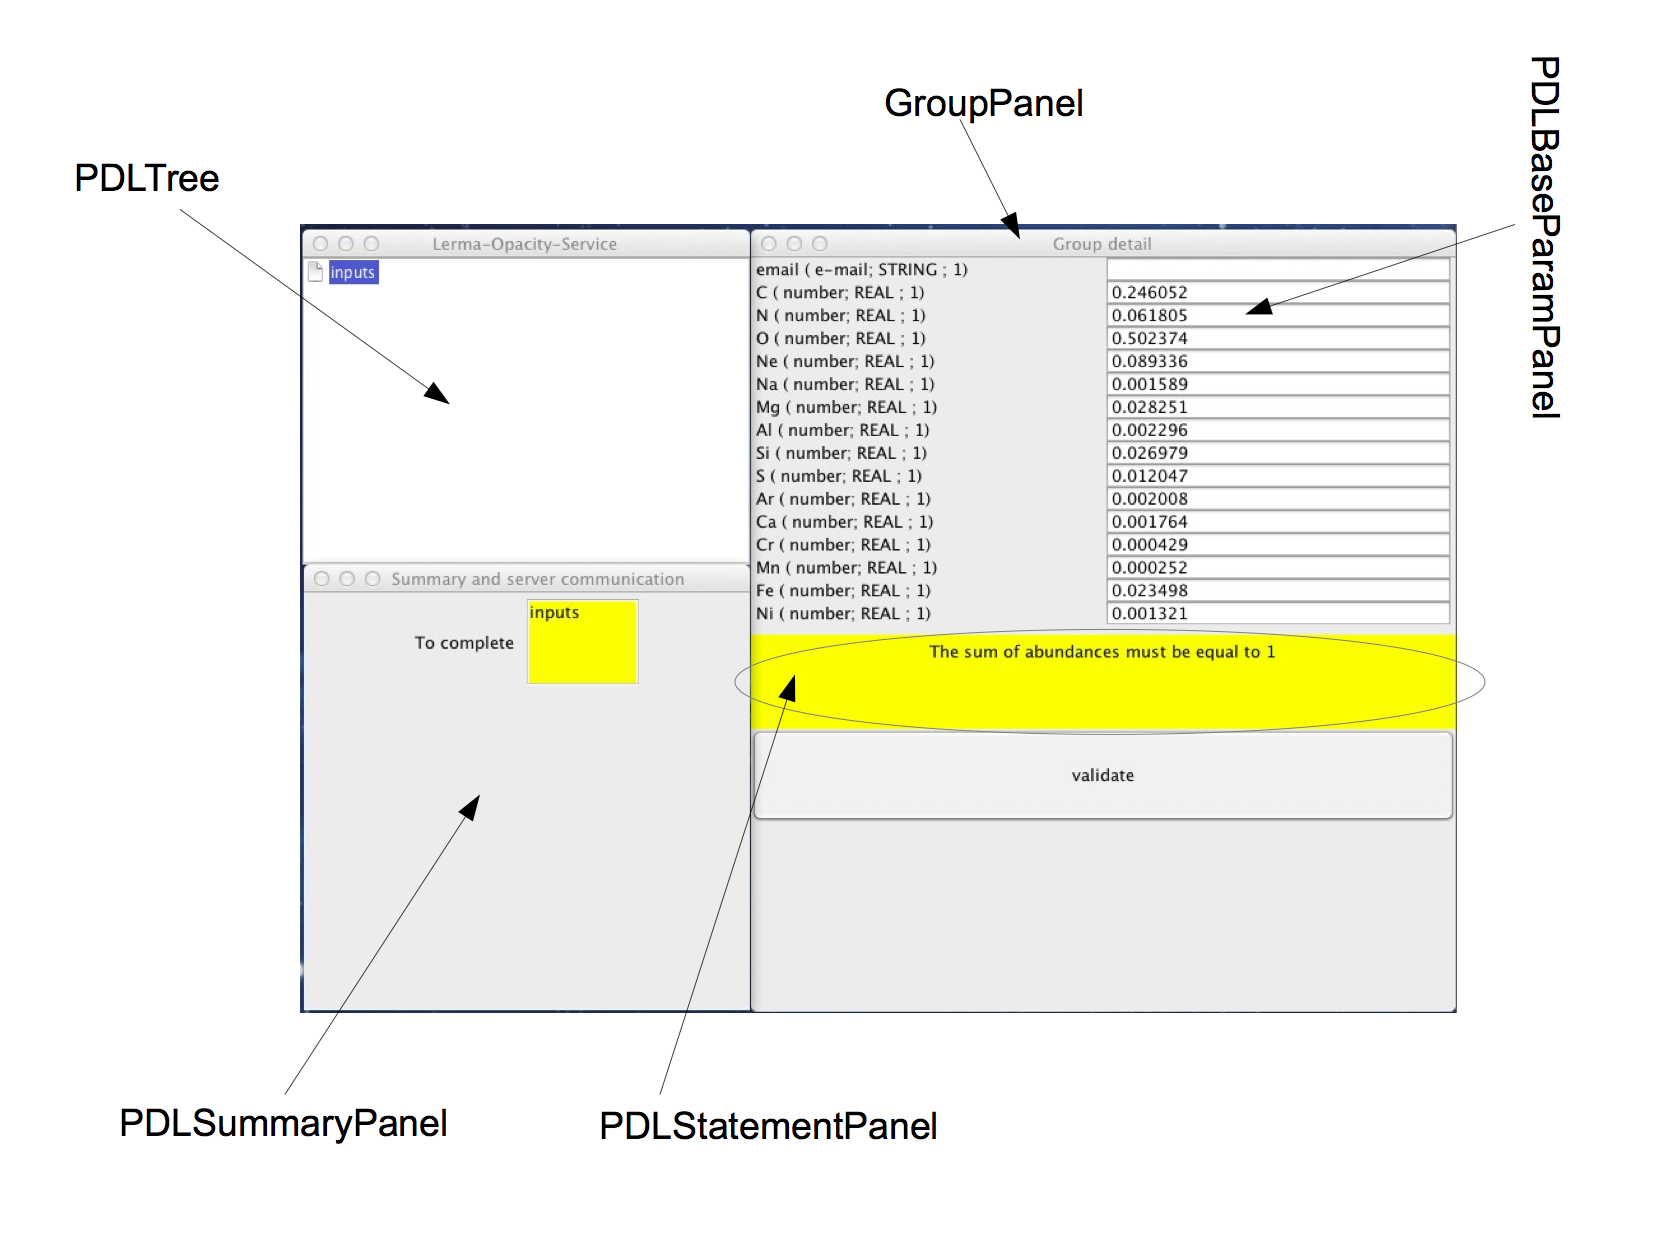
\includegraphics[width=1.2\textwidth]{pictures/PDLGui.jpg} 
\caption{PDL GUI with highlights of the macro graphical components corresponding to the classes of the present package}
\label{PDLGui.jpg}
\end{center}
\end{figure}

\section{The test package}
The class {\it BaseExample} and the classing inheriting from it (BroadeningExample, Example02, ExampleInteropPune02, OpacityExample, PDRExample, PDRService, Principale) are used only for generating using the Jax-B framework the instances of the PDL descriptions that will be interpreted by the dynamic GUI. Indeed they are {\it a priori} with respect to the mechanisms we have exposed in this document.\\

\noindent Starting from an instance of  PDL service description (contained into the file named PDL-Description.xml), the {\it buildService} method of the class {\it GUITest} (which takes no argument) uses the Jax-B framework and return a{\it Service} object containing the Java object structure corresponding to the transposition of the XML into Java objects (cf. par. \ref{Java_Objects}). This method is called by the {\it main} function of {\it GUITest} which, after this invocation,  will initialize the instance of {UserMapper} that will be used in all the application and will build an instance of {\it IntelligentGUI}  that will display the graphical interface.

\end{document}





 
